\documentclass{article}

\usepackage{amsmath}
\usepackage{amssymb}
\usepackage{amsfonts}
\usepackage{mathrsfs}
\usepackage{latexsym}
\usepackage{bm}
\usepackage[dvipdfmx]{graphicx}
\usepackage{physics}
\usepackage{braket}
\usepackage{float}



\title{Notes on density functional theory}
\author{Ryota Masuki}
\date{\today}

\begin{document}
\maketitle

\section{Pseudopotential methods}
\subsection{Projector Augmented Wave (PAW) method}
\subsubsection{Theory}
The all electron wavefunction $\ket{\Psi}$ is written by 
\begin{align}
\ket{\Psi} = \mathcal{T} \ket{\widetilde{\Psi}}
\end{align}
using the pseudo wavefunction $\ket{\widetilde{\Psi}}$. Here, the PAW transformation, which transforms the PS wavefunction to AE wavefunction, is 
\begin{align}
  \mathcal{T} = 1 + \sum_{\bm{R}\alpha} \mathcal{T}_{\bm{R}\alpha},
\end{align}
where $\mathcal{T}_{\bm{R}\alpha}$ operates in a sphere surrounding the atom $\bm{R}\alpha$.

Here, for a set of complete set in the sphere $\ket{\widetilde{\phi}_{\bm{R}\alpha, nL}}$, we assume that 
\begin{align}
  \ket{{\phi}_{\bm{R}\alpha, nL}} = (1 + \mathcal{T}_{\bm{R}\alpha}) \ket{\widetilde{\phi}_{\bm{R}\alpha, nL}}.
\end{align}
Then, using the projecor functions $\ket{\widetilde{p}_{\bm{R}\alpha,nL}}$, which satisfies
\begin{align} 
  \sum_{nL} \ket{\widetilde{\phi}_{\bm{R}\alpha, nL}} \bra{\widetilde{p}_{\bm{R}\alpha, nL}} = 1
\end{align}
for all atoms $\bm{R}\alpha$, the PAW transformation can be explicitly written as 
\begin{align}
  \mathcal{T} = 1 + \sum_{i = (\bm{R}\alpha, nL)} (\ket{\phi_i} - \ket{\widetilde{\phi}_i}) \bra{\widetilde{p}_i}.
\end{align}

\subsubsection{Operators}
For any one-body operator $A$, 
\begin{align}
  \widetilde{A} 
  &= \mathcal{T}^\dag A \mathcal{T}
  \\&=
  A + 
  \sum_{i = (\bm{R}_1\alpha_1,n_1L_1),j = (\bm{R}_2\alpha_2, n_2 L_2)}
  \ket{\widetilde{p}_i}
  (\braket{\phi_i | A | \phi_j} - 
  \braket{\widetilde{\phi}_i | A | \widetilde{\phi}_j})
  \bra{\widetilde{p}_j}
  + \Delta A
\end{align}
Please see Ref.~\cite{PhysRevB.50.17953} for details of $\Delta A$.
When $A$ is a semilocal operator, $\Delta A$ vanishes, and the second term can be rewritten as 
\begin{align}
  \widetilde{A} 
  &= \mathcal{T}^\dag A \mathcal{T}
  \\&=
  A + 
  \sum_{\bm{R}\alpha,n_1L_1, n_2 L_2}
  \ket{\widetilde{p}_{\bm{R}\alpha,n_1L_1}}
  (\braket{\phi_{\bm{R}\alpha,n_1L_1} | A | \phi_{\bm{R}\alpha,n_2L_2}} - 
  \braket{\widetilde{\phi}_{\bm{R}\alpha,n_1L_1} | A | \widetilde{\phi}_{\bm{R}\alpha,n_2L_2}})
  \bra{\widetilde{p}_{\bm{R}\alpha,n_2L_2}}
\end{align}
The charge density is given by
\begin{align}
  n(\bm{r}) = \widetilde{n}(\bm{r}) + n^1(\bm{r}) - \widetilde{n}^1(\bm{r}),
\end{align}
where
\begin{align}
\widetilde{n}(\bm{r}) =  \sum_{n\bm{k}} f_{n\bm{k}} |\widetilde{\psi}_{n\bm{k}}(\bm{r})|^2 
\end{align}
\begin{align}
  {n}^1(\bm{r}) =  \sum_{n\bm{k}} \sum_{\bm{R}\alpha, nL, n'L'} f_{n\bm{k}} 
  \braket{\widetilde{\psi}_{n\bm{k}} | \widetilde{p}_{\bm{R}\alpha, nL}} 
  \phi^*_{\bm{R}\alpha, nL}(\bm{r})
  \phi^*_{\bm{R}\alpha, n'L'}(\bm{r})
  \braket{ \widetilde{p}_{\bm{R}\alpha, n'L'} | \widetilde{\psi}_{n\bm{k}} } 
\end{align}
\begin{align}
  \widetilde{n}^1(\bm{r}) =  \sum_{n\bm{k}} \sum_{\bm{R}\alpha, nL, n'L'} f_{n\bm{k}} 
  \braket{\widetilde{\psi}_{n\bm{k}} | \widetilde{p}_{\bm{R}\alpha, nL}} 
  \widetilde{\phi}^*_{\bm{R}\alpha, nL}(\bm{r})
  \widetilde{\phi}^*_{\bm{R}\alpha, n'L'}(\bm{r})
  \braket{ \widetilde{p}_{\bm{R}\alpha, n'L'} | \widetilde{\psi}_{n\bm{k}} } 
\end{align}

\begin{figure}[H]
  \begin{center}
  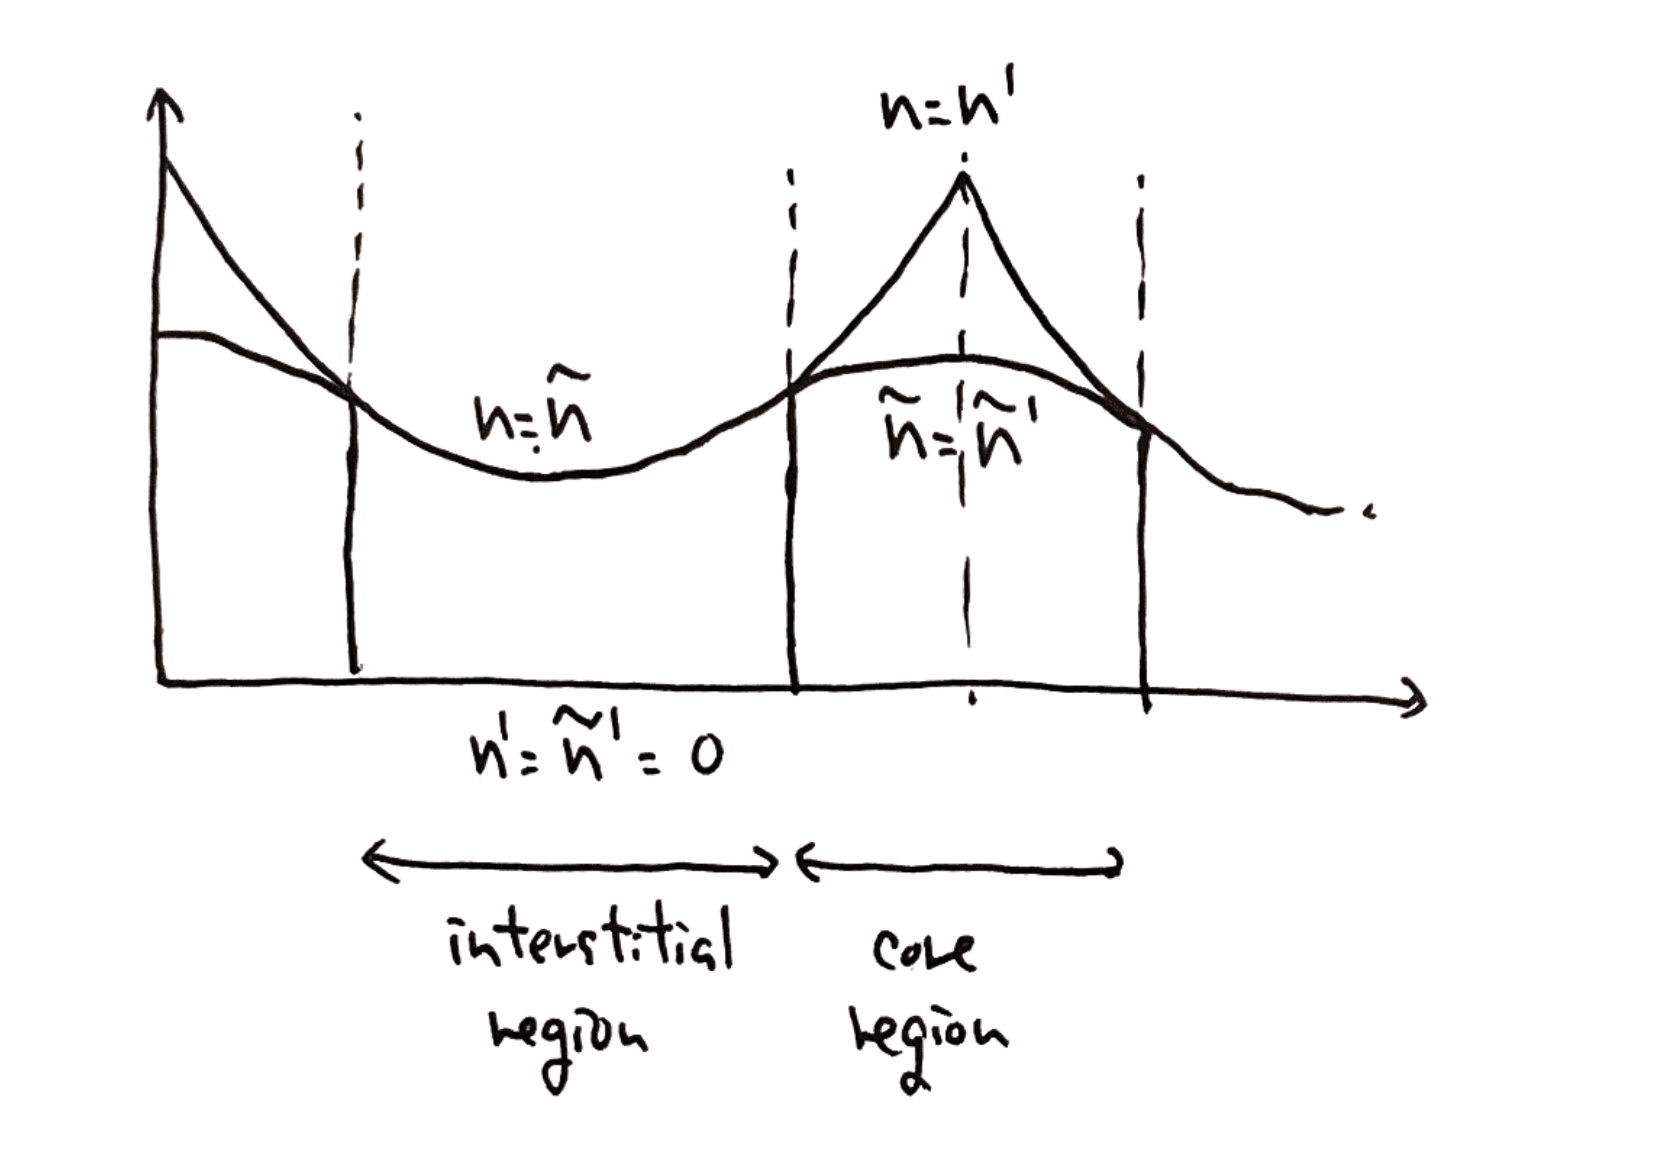
\includegraphics[width=100mm]{figures/PAW_charge.png}
  \caption{Schematic of the PAW charge densities.}
  \end{center}
\end{figure}

\subsubsection{Total energy}
Under LDA, the total energy functional is 
\begin{align}
  E &=
  \sum_{n\bm{k}} f_{n\bm{k}} \braket{\phi_{n\bm{k}} | \frac{-\hbar^2\nabla^2}{2m} | \phi_{n\bm{k}}}
  \nonumber
  \\&+
  \frac{e^2}{2} \int d\bm{r}d\bm{r}' \frac{(n(\bm{r})+ n^Z(\bm{r})) (n(\bm{r}')+ n^Z(\bm{r}'))}{|\bm{r} - \bm{r}'|}
  + \int d\bm{r} n(\bm{r})\epsilon_{xc}(n(\bm{r})),
\end{align}
where $n^Z$ is the (charge) density of nuclei in the unit of $-e$.
With a cumbersome calculation, we can prove that $E = \widetilde{E} + E^1 - \widetilde{E}^1$ with
\begin{align} 
  \widetilde{E} &= 
  \sum_{n\bm{k}} f_{n\bm{k}} \braket{\widetilde{\psi}_{n\bm{k}} | \frac{-\hbar^2\nabla^2}{2m} |\widetilde{\psi}_{n\bm{k}} }
  + \frac{e^2}{2}\int d\bm{r}d\bm{r}' \frac{(\widetilde{n} + \hat{n})(\widetilde{n} + \hat{n})}{|\bm{r}-\bm{r}'|}
  \nonumber \\&
  + \int d\bm{r} \widetilde{n}(\bm{r})\bar{v}(\bm{r})
  + \int d\bm{r} \widetilde{n}(\bm{r})\epsilon_{xc}(\widetilde{n}(\bm{r})),
  \label{eq:tildeE}
\end{align}
\begin{align} 
  {E}^1 &= 
  \sum_{n\bm{k}} \sum_{\bm{R}\alpha, nL, n'L'}f_{n\bm{k}} 
  \braket{\widetilde{\psi}_{n\bm{k}} | \widetilde{p}_{\bm{R}\alpha, nL}}
  \braket{\phi_{\bm{R}\alpha, nL}| \frac{-\hbar^2\nabla^2}{2m} |\phi_{\bm{R}\alpha, n'L'}}
  \braket{\widetilde{p}_{\bm{R}\alpha, n'L'}|\widetilde{\psi}_{n\bm{k}} }
  \nonumber\\&
  + \frac{e^2}{2}\int d\bm{r}d\bm{r}' \frac{({n}^1 + n^Z)({n}^1 + n^Z)}{|\bm{r}-\bm{r}'|}
  + \int d\bm{r} {n}^1(\bm{r})\epsilon_{xc}({n}^1(\bm{r})),
\end{align}
\begin{align} 
  \widetilde{E}^1 &= 
  \sum_{n\bm{k}} \sum_{\bm{R}\alpha, nL, n'L'}f_{n\bm{k}} 
  \braket{\widetilde{\psi}_{n\bm{k}} | \widetilde{p}_{\bm{R}\alpha, nL}}
  \braket{\widetilde{\phi}_{\bm{R}\alpha, nL}| \frac{-\hbar^2\nabla^2}{2m} |\widetilde{\phi}_{\bm{R}\alpha, n'L'}}
  \braket{\widetilde{p}_{\bm{R}\alpha, n'L'}|\widetilde{\psi}_{n\bm{k}} }
  \nonumber\\&
  + \frac{e^2}{2}\int d\bm{r}d\bm{r}' \frac{(\widetilde{n}^1 + \hat{n})(\widetilde{n}^1 + \hat{n})}{|\bm{r}-\bm{r}'|}
  + \int d\bm{r} \widetilde{n}^1(\bm{r})\bar{v}(\bm{r})
  + \int d\bm{r} \widetilde{n}^1(\bm{r})\epsilon_{xc}(\widetilde{n}^1(\bm{r})).
\end{align}
Note that 
\begin{itemize}
  \item $\bar{v}$ is arbitrary potential which vanishes in the interstitial region.
  \item $\hat{n}$ is the compensation charge density that cannot be distinguished from $n + n^Z - \widetilde{n} = n^1 + n^Z - \widetilde{n}^1$ when seen from the interstitial region. $\widetilde{n} + \hat{n}$ is a smooth charge density with charge neutrality. ${n}^1 + n^Z$ in $E^1$ and $\ widetilde{n}^1 + \hat{n}$ in $\widetilde{E}^1$ are confined in the core region. These densities have the same charge as the charge in the core region. These Coulomb integrals in $E^1$ and $\widetilde{E}^1$ are infinite, but the divergent term cancel with each other.
\end{itemize}
The compenastion charge  desnity $\hat{n}$ is determined as
\begin{align}
  \hat{n}_{\bm{R}\alpha} = \sum_L g_{\bm{R}\alpha L}(\bm{r}) Q_{\bm{R}\alpha L},
\end{align}
\begin{align}
  g_{\bm{R}\alpha L} = 
  C_{\alpha l} |\bm{r} - \bm{R}_{\alpha} |^l  Y_{L}(\widehat{\bm{r} - \bm{R}_{\alpha}}) 
  \exp \Bigl( - \frac{|\bm{r} - \bm{R}|^2}{r_{c\alpha}^2} \Bigr),
\end{align}
\begin{align}
  Q_{\bm{R}\alpha L} = \int d\bm{r} |\bm{r} - \bm{R}_{\alpha}|^l (n^1(\bm{r}) + \bm{n}^Z(\bm{r}) - \widetilde{n}^1(\bm{r})) Y^*_L (\widehat{\bm{r} - \bm{R}_{\alpha}}),
\end{align}
so that $\hat{n}$ has the same multipole moments as $n^1 + \bm{n}^Z - \widetilde{n}^1$.
$C_{l\alpha}$ is the normalization constant so that
\begin{align}
  &
  C_{\alpha l} \int d\bm{r} |\bm{r} - \bm{R}_{\alpha}|^l Y^*_{L}(\widehat{\bm{r} - \bm{R}_{\alpha}}) g_{\bm{R}\alpha L}(\bm{r})
  \\&=
  C_{\alpha l} \int_0^{r_{c\alpha}} r^{2l+2}e^{-r^2/r_{c\alpha}^2} = 1
\end{align}
is satisfied. In the limit of $r_{c\alpha} \to \infty$, 
\begin{align}
  C_{\alpha l} \to \frac{2}{r_{c\alpha}^{2l+3} \Gamma(\frac{2l+3}{2})}.
\end{align}

\subsubsection{Methods for numerical calculations}
The second term in the RHS of Eq. (\ref{eq:tildeE}) can be calculated by using another compensation charge density
\begin{align}
  \hat{n}'_{\bm{R}\alpha} = \sum_L g'_{\bm{R}\alpha L}(\bm{r}) Q_{\bm{R}\alpha L},
\end{align}
which has the same multipole moment as $\hat{n}$. With $\hat{n}'$.
We choose $\hat{n}'$ is smooth enough so that its high-frequency components are negligible. 
Then, the second term in the RHS of Eq. (\ref{eq:tildeE}) can be rewritten as 
\begin{align}
  &
\frac{e^2}{2}\int d\bm{r}d\bm{r}' \frac{(\widetilde{n} + \hat{n})(\widetilde{n} + \hat{n})}{|\bm{r}-\bm{r}'|}
\nonumber
\\&=
\frac{e^2}{2}\int d\bm{r}d\bm{r}' \frac{(\widetilde{n} + \hat{n}')(\widetilde{n} + \hat{n}')}{|\bm{r}-\bm{r}'|}
\label{eq:Coulomb_tn_hn_1}
\\&
+
\int d\bm{r} \widetilde{n} (\bm{r}) \hat{v}(\bm{r})
\label{eq:Coulomb_tn_hn_2}
\\&
+ 
\sum_{\bm{R}\alpha, \bm{R}'\alpha'} U_{\bm{R}\alpha,\bm{R}'\alpha'},
\end{align}
where
\begin{align}
  \hat{v}(\bm{r}) = e^2 \int d\bm{r}' \frac{ \hat{n}(\bm{r}') - \hat{n}'(\bm{r}')}{|\bm{r}-\bm{r}'|},
\end{align}
and
\begin{align}
  U_{\bm{R}\alpha,\bm{R}'\alpha'} 
  = \frac{e^2}{2}\int_A d\bm{r}d\bm{r}' \frac{\hat{n}_{\bm{R}\alpha}\hat{n}_{\bm{R}\alpha} - \hat{n}'_{\bm{R}\alpha} \hat{n}'_{\bm{R}\alpha}}{|\bm{r}-\bm{r}'|},
  \label{eq:U_RaRpap}
\end{align}
where $\int_A$ means that some analytical formulas are used to estimate the integral (I haven't checked the details).
Eq. (\ref{eq:Coulomb_tn_hn_1}) can be estimated in the Fourier space
\begin{align}
  &
  \frac{e^2}{2}\int_M d\bm{r}d\bm{r}' \frac{(\widetilde{n} + \hat{n}')(\widetilde{n} + \hat{n}')}{|\bm{r}-\bm{r}'|}
  \\&=
  N\times \frac{2\pi}{\Omega_{\text{cell}}} \sum_{|\bm{G}| < G_{\text{cutoff}} } \frac{|(\widetilde{n} + \hat{n}')_{\bm{G}}|^2}{G^2}.
  \label{eq:intM_Coulomb_tn_hnp}
\end{align}
Here, $\int_M$ is a integral on Fourier mesh, we define the LHS integral as the sum of RHS.
Although $\hat{v}$ in Eq. (\ref{eq:Coulomb_tn_hn_2}) includes high-frequency components, it can be written as
\begin{align}
  \int_M d\bm{r} \widetilde{n} (\bm{r}) \hat{v}(\bm{r}) 
  =
  N\times \frac{2\pi}{\Omega_{\text{cell}}} \sum_{|\bm{G}| < G_{\text{cutoff}} } \frac{\widetilde{n}_{\bm{G}}(\hat{n} - \hat{n}')_{-\bm{G}}}{G^2}.
  \label{eq:intM_tn_hv}
\end{align}
because the high-frequency components of $\widetilde{n}$ vanish.
Note that the convention of the Fourier transofrmation of the charge density is
\begin{align}
  n_{\bm{G}} &= \int_{\text{cell}}d \bm{r} e^{-i\bm{G}\cdot \bm{r}} n(\bm{r})
  \\
  n(\bm{r}) &= \frac{1}{\Omega_{\text{cell}}} \sum_{\bm{G}} e^{i\bm{G}\cdot \bm{r}} n_{\bm{G}} 
\end{align}
Summrizing above, we get
\begin{align} 
  \widetilde{E} &= 
  \sum_{n\bm{k}} f_{n\bm{k}} \braket{\widetilde{\psi}_{n\bm{k}} | \frac{-\hbar^2\nabla^2}{2m} |\widetilde{\psi}_{n\bm{k}} }
  \nonumber
  \\&
  + \frac{e^2}{2}\int_M d\bm{r}d\bm{r}' \frac{(\widetilde{n} + \hat{n}')(\widetilde{n} + \hat{n}')}{|\bm{r}-\bm{r}'|}
  + \int_M d\bm{r} \widetilde{n} (\bm{r}) \hat{v}(\bm{r}) 
  + \sum_{\bm{R}\alpha, \bm{R}'\alpha'} U_{\bm{R}\alpha,\bm{R}'\alpha'},
  \nonumber
  \\&
  + \int_M d\bm{r} \widetilde{n}(\bm{r})\bar{v}(\bm{r})
  + \int_M d\bm{r} \widetilde{n}(\bm{r})\epsilon_{xc}(\widetilde{n}(\bm{r})),
  \label{eq:tildeE_numerical_calculation}
\end{align}
where the explicit formulas for the terms with $\int_M$ are defined in Eqs. (\ref{eq:intM_Coulomb_tn_hnp}) and (\ref{eq:intM_tn_hv}). $U_{\bm{R}\alpha,\bm{R}'(\alpha')}$ is defined in Eq. (\ref{eq:U_RaRpap}).
The last two terms can also be estimated with an integral on the Fourier mesh like Eq. (\ref{eq:intM_tn_hv}).
\begin{align} 
  {E}^1 &= 
  \sum_{n\bm{k}} \sum_{\bm{R}\alpha, nL, n'L'}f_{n\bm{k}} 
  \braket{\widetilde{\psi}_{n\bm{k}} | \widetilde{p}_{\bm{R}\alpha, nL}}
  \braket{\phi_{\bm{R}\alpha, nL}| \frac{-\hbar^2\nabla^2}{2m} |\phi_{\bm{R}\alpha, n'L'}}
  \braket{\widetilde{p}_{\bm{R}\alpha, n'L'}|\widetilde{\psi}_{n\bm{k}} }
  \nonumber\\&
  + \frac{e^2}{2}\int_{RG} d\bm{r}d\bm{r}' \frac{({n}^1 + n^Z)({n}^1 + n^Z)}{|\bm{r}-\bm{r}'|}
  + \int_{RG} d\bm{r} {n}^1(\bm{r})\epsilon_{xc}({n}^1(\bm{r})),
\end{align}
\begin{align} 
  \widetilde{E}^1 &= 
  \sum_{n\bm{k}} \sum_{\bm{R}\alpha, nL, n'L'}f_{n\bm{k}} 
  \braket{\widetilde{\psi}_{n\bm{k}} | \widetilde{p}_{\bm{R}\alpha, nL}}
  \braket{\widetilde{\phi}_{\bm{R}\alpha, nL}| \frac{-\hbar^2\nabla^2}{2m} |\widetilde{\phi}_{\bm{R}\alpha, n'L'}}
  \braket{\widetilde{p}_{\bm{R}\alpha, n'L'}|\widetilde{\psi}_{n\bm{k}} }
  \nonumber\\&
  + \frac{e^2}{2}\int_{RG} d\bm{r}d\bm{r}' \frac{(\widetilde{n}^1 + \hat{n})(\widetilde{n}^1 + \hat{n})}{|\bm{r}-\bm{r}'|}
  + \int_{RG} d\bm{r} \widetilde{n}^1(\bm{r})\bar{v}(\bm{r})
  + \int_{RG} d\bm{r} \widetilde{n}^1(\bm{r})\epsilon_{xc}(\widetilde{n}^1(\bm{r})),
\end{align}
where $RG$ stands for radial grid integration. $\int_{RG}$ for terms like $\int_{RG} d\bm{r} n(\bm{r})\epsilon_{xc}(n(\bm{r}))$ are defined as Eq. (29) in Ref.~\cite{PhysRevB.50.17953}. 
It seems that the Coulom integrals for $({n}^1 + n^Z)$ and $(\widetilde{n}^1 + \hat{n})$ can be estimated using a radial grid integration, but I haven't confirmed the exact details.  
I haven't followed the details of $\int_{RG} d\bm{r} \widetilde{n}^1(\bm{r})\bar{v}(\bm{r})$ as well, which I suppose depends on how to determine $\bar{v}$.

\bibliographystyle{unsrt}
\bibliography{reference}
\end{document}